% Тут используется класс, установленный на сервере Papeeria. На случай, если
% текст понадобится редактировать где-то в другом месте, рядом лежит файл matmex-diploma-custom.cls
% который в момент своего создания был идентичен классу, установленному на сервере.
% Для того, чтобы им воспользоваться, замените matmex-diploma на matmex-diploma-custom
% Если вы работаете исключительно в Papeeria то мы настоятельно рекомендуем пользоваться
% классом matmex-diploma, поскольку он будет автоматически обновляться по мере внесения корректив
%

% По умолчанию используется шрифт 14 размера. Если нужен 12-й шрифт, уберите опцию [14pt]
\documentclass[12pt]{matmex-diploma}
%\documentclass{matmex-diploma-custom}
\newfontfamily{\cyrillicfonttt}{Liberation Mono}
\usepackage{verbatim}
\usepackage{float}
\usepackage{caption}
\usepackage{subcaption}
\usepackage{graphicx}
\usepackage{minted}
\usepackage{verbments}
\usepackage{array}
\usepackage{semantic}
\usepackage{stmaryrd}
\usepackage{listings}


\renewcommand\listingscaption{Листинг}
\renewcommand{\lstlistingname}{Листинг}
\newcommand \bnfdef  {\mathrel{::=}}
\newcommand \bnfalt  {\mathrel{{|}}}
\newcommand \lpar  {\mathrel{{[}}}
\newcommand \rpar  {\mathrel{{]}}}
\newcommand \llpar  {\mathrel{{\llbracket}}}
\newcommand \rrpar  {\mathrel{{\rrbracket}}}
 
\begin{document}
% Год, город, название университета и факультета предопределены,
% но можно и поменять.
% Если англоязычная титульная страница не нужна, то ее можно просто удалить.
\filltitle{ru}{
    chair              = {Математическое обеспечение и администрирование\\ информационных систем\\
                           \vskip 1em
                          Системное программирование},
    title              = {Компиляция сертифицированных F*-программ в робастные Web-приложения},
    % Здесь указывается тип работы. Возможные значения:
    %   coursework - Курсовая работа
    %   diploma - Диплом специалиста
    %   master - Диплом магистра
    %   bachelor - Диплом бакалавра
    type               = {master},
    position           = {студента},
    group              = 646,
    author             = {Полубелова Марина Игоревна},
    supervisorPosition = {к.\,ф.-м.\,н., доцент},
    supervisor         = {Григорьев С.\,В.},
    reviewerPosition   = { OOO ``ИнтеллиДжей Лабс''\\ разработчик ПО},
    reviewer           = {Мордвинов Д.\,А.},
    chairHeadPosition  = {д.\,ф.-м.\,н., профессор},
    chairHead          = {Терехов А.\,Н.}
%   university         = {Санкт-Петербургский Государственный Университет},
%   faculty            = {Математико-механический факультет},
%   city               = {Санкт-Петербург},
%   year               = {2013}
}
\filltitle{en}{
    type               = {master},
    chair              = {Software and Administration of Information Systems\\
                          \vskip 1em
                          Software Engineering},
    title              = {Compiling Verified F* Programs to Robust Web Applications},
    author             = {Polubelova Marina},
    supervisorPosition = {Associate Professor},
    supervisor         = {Grigorev S.\,V.},
    reviewerPosition   = {``IntelliJ Labs Co.Ltd''\\ Software Developer},
    reviewer           = {Mordvinov D.\,A.},
    chairHeadPosition  = {professor}, 
    chairHead          = {Terekhov A.\,N.},
    city               = {Saint-Petersburg} 
}
\maketitle
\tableofcontents
% У введения нет номера главы
\section*{Введение}

В последнее время происходит стремительный рост количества устройств, подключаемых к Интернет. Взаимодействие между этими устройствами осуществляется с использованием различных протоколов. В зависимости от целей и потребностей пользователей Интернет-устройств формулируются различные требования к таким протоколам. Одно из важных требований является обеспечение конфиденциальности и целостности пользовательских данных. Например, при оплате онлайн-покупок банковской картой покупатель хочет быть уверен в том, что данные его карты не попадут к злоумышленникам, а банк получит именно те данные, которые были введены пользователем. Безопасность соединения таких Интернет-устройств зависит от используемых криптографических протоколов и кода Веб-приложений, который чаще всего создается на JavaScript~\cite{js_semantics}. Поэтому необходимо гарантировать безопасность используемых протоколов и Веб-приложений, а для последних еще и робастность (robustness). Веб-приложение является робастным, если оно продолжает работу даже при неверных входных данных, а не завершается аварийно. 

Для работы Веб-приложений широко используется криптографический протокол Transport Layer Security (TLS)~\cite{tls}, который обеспечивает защищенную передачу данных. Для установки соединения между клиентом и сервером протокол сначала выполняет процедуру подтверждения сеанса связи, которая включает в себя согласование используемых алгоритмов шифрования и хэш-функций, валидацию сертификата сервера. После этого протокол устанавливает безопасное соединение, которое обеспечивает конфиденциальность передаваемых данных. Для сохранения целостности и аутентификации сообщений используются так называемые коды аутентификации --- дополнительная  информация, получаемая на основе передаваемых данных и позволяющая доказать, что сообщение не изменилось и не было подделано. Несмотря на продолжительное время разработки криптографических библиотек (например, библиотека OpenSSL~\cite{openssl} разрабатывается с 1998 года), они остаются подвержены хакерским атакам. При этом многие атаки используют ошибки, допущенные в программном обеспечении. Например, ставшая известной в  2014 году уязвимость Heartbleed~\cite{heartbleed} в криптографической библиотеке OpenSSL позволяла несанкционированное чтение памяти на сервере или на клиенте.

Итак, существует необходимость в создании надежных систем, которые будут устойчивы к хакерским атакам. С одной стороны, для этого нужны новые протоколы, с другой --- необходимы новые подходы к разработке программного обеспечения. Одним из таких подходов является использование сертифицированного программирования~\cite{certifiedProgramming} для создания и верификации программ, которые затем транслируются в целевой язык. Сертифицированное программирование позволяет доказывать, что программа соответствует своему формальному описанию. Данный процесс происходит статически, что позволяет гарантировать, что программа всегда работает так, как указано в ее спецификации. В качестве инструментов для создания сертифицированных программ используются такие инструменты как Coq~\cite{coq}, Agda~\cite{agda}, F*~\cite{fstar}, Idris~\cite{idris} и другие.  При этом необходимо гарантировать, что весь стек от создания программы до получения целевого кода является корректным и безопасным, так же, как и полученная в результате этого программа. 

Данный подход применяется в проекте Everest~\cite{everest}, который нацелен на создание высокопроизводительной, соответствующей спецификациям, реализации протокола HTTPS. Данные в этом протоколе передаются поверх криптографического протокола TLS. Данный проект включает в себя подпроекты miTLS~\cite{mitls} и HACL*~\cite{hacl_star}, которые посвящены верификации, соответственно, протокола TLS и криптографических примитивов. Для создания и верификации программ выбран функциональный язык программирования F*~\cite{fstarCite}. С одной стороны, этот язык обладает богатой системой типов, которая включает в себя зависимые (dependent types) и уточняющие типы (refinement types)~\cite{certifiedProgramming}. С другой стороны, F* позволяет доказывать многие свойства программы, например, что эффективная реализация программы соответствует своей спецификации. Для F* разработаны механизмы извлечения верифицированного кода в программы на OCaml и C~\cite{kremlin}. Данный подход обеспечивает относительную независимость процесса создания программы от целевой платформы, позволяя использовать проверифицированный код во многих областях. 

В данной работе целевым языком для компиляции F*-программ выбран JavaScript. Данный язык поддерживается всеми современными Веб-браузерами, не требуя установки дополнительного программного обеспечения. В данной работе предложены правила трансляции с языка F* в JavaScript (ECMAScript~6~\cite{specjs}), гарантирующие сохранение аннотации типов. Это позволяет эффективно использовать инструмент Flow~\cite{flow} (статический анализатор типов для JavaScript) для дополнительной проверки оттранслированной программы. %В рамках данной работы было также проведено экспериментальное исследование реализованного инструмента на примерах из F* tutorial~\cite{fstar} и криптографической библиотеке HACL*~\cite{hacl_star}.

Данная работа была инициирована в рамках стажировки автора в INRIA Paris под руководством Karthikeyan Bhargavan. Проводимые исследования были поддержаны грантом JetBrains Research.

\section{Постановка задачи}
Целью данной работы является разработка инструмента для компиляции сертифицированных F*-программ в робастные Web-приложения на JavaScript. Для ее достижения были поставлены следующие задачи:

\begin{itemize}
\item сформулировать правила трансляции с языка F* на JavaScript, гарантирующие сохранение аннотаций типов;
\item выполнить реализацию предложенного подхода;
\item провести экспериментальное исследование реализованного инструмента.
\end{itemize} 

\section{Обзор}

В данном обзоре описаны исходный и целевой языки трансляции, а именно, языки программирования F* и JavaScript. Описан инструмент Flow, используемый в работе, а также приведено обоснование выбора данного инструмента. Приведено также описание существующих инструментов для трансляции OCaml-программ в JavaScript-приложения. В конце обзора дано описание проекта HACL*, который является контекстом данной работы и из которого были взяты тестовые данные для проведения экспериментального исследования инструмента, реализованного в рамках данной работы. 

\subsection{Язык F*}

В данной работе исходным языком для трансляции программ является функциональный язык программирования F*~\cite{fstargh, fstarCite, fstar}, который ориентирован на верификацию программ. Система типов F* включает в себя полиморфизм, уточняющие и зависимые типы (refinement and dependent types), monadic effects и вычисление слабейших предусловий. Данный язык позволяет создавать и верифицировать программы, то есть доказывать, что программа соответствует своей спецификации. Для этого данный инструмент использует SMT-решатель Z3~\cite{z3Cite} и доказательства, написанные пользователем. Проверифицированный код можно извлечь в программы на OCaml и C~\cite{kremlin}. 

Для того чтобы продемонстрировать основные особенности языка F*, рассмотрим пример вычисления факториала (см. листинг~\ref{lst:fact1}). 

\begin{listing}
\begin{pyglist}[language=ocaml,numbers=none,numbersep=5pt, fontsize=\small]
let rec fact n =
    if n = 0 then 1 else n * (fact (n - 1))  
\end{pyglist}
\caption{Функция вычисления факториала}
\label{lst:fact1}  
\end{listing}

Для функции \verb|fact| система типов языка F* выведет тип $int ~\to~ int$. Данная программа работает корректно для всех неотрицательных чисел, но если вызвать данную функцию от отрицательного аргумента, например, \verb|fact -2|, то программа зациклится. Чтобы избежать такой ситуации, можно ввести ограничения на входные параметры функции. Сделать это можно с использованием уточняющих типов (см. листинг~\ref{lst:fact2}).

\begin{listing} 
\begin{pyglist}[language=ocaml,numbers=none,numbersep=5pt, fontsize=\small]
val fact: x:int{x >= 0} -> Tot int
let rec fact n =
    if n = 0 then 1 else n * (fact (n - 1))  
\end{pyglist}
\caption{Функция вычисления факториала с эффектом $Tot$}
\label{lst:fact2}   
\end{listing}

Уточняющие типы имеют вид $x:t\{phi(x)\}$, где элемент $x$ принадлежит к типу $t$ и удовлетворяет предикату $phi(x)$. В данном примере таким типом является \verb|x:int{x >= 0}|. В этом же примере появилось ключевое слово $Tot$ (total), которое отражает эффект вычисления функции. Данный эффект ($Tot~t$) гарантирует, что функция всегда завершает работу, а полученный результат имеет тип $t$. Когда в программе происходит вызов данной функции, то при верификации проверяется, что аргументы вызывающей функции удовлетворяют ее условиям.

Для доказательства корректности программ можно использовать леммы, которые не имеют вычислительного эффекта и всегда возвращают \verb|unit|, но они позволяют доказывать многие свойства программы. При этом формулировка леммы ``находится'' в типах, а само доказательство приводится в теле функции. Например, можно доказать, что результат вычисления функции факториала числа всегда является положительным числом (см. листинг~\ref{lst:fact3}).

\begin{listing}
\begin{pyglist}[language=ocaml,numbers=none,numbersep=5pt, fontsize=\small]
val fact_property: x:int{x>=0} -> GTot (u:unit{fact x > 0})
let rec fact_property x =
   match x with
   | 0 -> ()
   | _ -> fact_property (x - 1)
\end{pyglist}
\caption{Результат вычисления факториала является положительным числом}
\label{lst:fact3} 
\end{listing}

Доказывается данное свойство индукцией по числу $x$. В данном примере используется ключевое слово $GTot$ (ghost total), которое как раз и означает, что функция не имеет вычислительного эффекта и всегда возвращает тип \verb|unit| (ghost-вычисления). При трансляции таких функций сохраняется только их сигнатура (уточняющие и зависимые типы заменяются на близкие им типы в целевом языке), при этом тело самой функции удаляется. Результат трансляции данного примера представлен в листинге~\ref{lst:fact4}.

\begin{listing}
\begin{pyglist}[language=ocaml,numbers=none,numbersep=5pt, fontsize=\small]
let fact_property (x:int) = ()
\end{pyglist}
\caption{Результат трансляции функции $fact\_property$}
\label{lst:fact4} 
\end{listing}

В данном примере используется зависимый тип \verb|u:unit{fact x > 0}|, который в общем случае имеет  вид $x:t_1 \to \ldots \to x_n:t_n [x_1 \ldots x_{n-1}] \to E~t [x_1 \ldots x_n]$. Нотация $t [x_1 \ldots x_{n-1}]$ означает, что переменные $x_1 \ldots x_{n-1}$ могут свободно входить в аргумент $t$. $E$ содержит эффект вычисления тела функции.

Данная функция может быть записана в виде, представленном в листинге~\ref{lst:fact5}, где ключевые слова \verb|requires| и \verb|ensures| соответствуют предусловию и постусловию леммы.

\begin{listing}
\begin{pyglist}[language=ocaml,numbers=none,numbersep=5pt, fontsize=\small]
val fact_property: x:int -> Lemma
    (requires (x >= 0))
    (ensures (fact x > 0))
let rec fact_property x =
   match x with
   | 0 -> ()
   | _ -> fact_property (x - 1)
\end{pyglist}
\caption{Результат вычисления факториала является положительным числом}
\label{lst:fact5} 
\end{listing}

Как уже было сказано, если не накладывать ограничения на входные параметры функции, то при вызове функции с отрицательным аргументом программа зациклится. Данный эффект можно отобразить с использованием ключевого слова $Dv$ (см. листинг~\ref{lst:fact6}).

\begin{listing}
\begin{pyglist}[language=ocaml,numbers=none,numbersep=5pt, fontsize=\small]
val fact : int -> Dv int 
let rec fact n =
    if n = 0 then 1 else n * (fact (n - 1))
\end{pyglist}
\caption{Функция вычисления факториала с эффектом $Dv$}
\label{lst:fact6} 
\end{listing}

Функцию вычисления факториала числа также можно написать с использованием ссылочных переменных (см. листинг~\ref{lst:fact7}), которые фактически являются указателями. Для обращения к хранимому значению используется нотация $!x$, для изменения хранимого значения --- $x1~:=~x2$. Ключевое слово $ST$ (stateful) означает, что выполнение функции происходит с использованием кучи, то есть могут выполняться операции чтения и записи, создания новых ссылочных переменных и т.д. Так как для вычислений используется куча, то необходима модель памяти, которая позволит доказывать необходимые свойства. Например, что два разных указателя не ссылаются на одну и ту же память (alias analysis). В данном примере $upd~h0~r1~x$ означает, что нужно обновить значение переменной по адресу $r1$ в куче $h0$ значением $x$. Конструкция $sel~h0~r1$ означает, что нужно выбрать значение, находящееся по адресу $r1$ в куче $h0$. Постусловие \verb|ensures| утверждает, что существует такое $x$, что в результате выполнения функции \verb|fact_st| в куче $h1$ будет содержаться результат выполнения функции \verb|fact x| (так как $sel~h0~r1~=~x$) по адресу $r2$.

\begin{listing}
\begin{pyglist}[language=ocaml,numbers=none,numbersep=5pt, fontsize=\small]
type nat = x:int{x>=0} 

val fact_st : r1:ref nat -> r2:ref nat -> ST unit
    (requires (fun h0 -> True))
    (ensures (fun h0 _ h1 -> 
    exists x. h1 == (upd (upd h0 r1 x) r2 (fact (sel h0 r1)))))
let rec fact_st r1 r2 =
  let x1 = !r1 in
  if x1 = 0 
  then r2 := 1
  else
     r1 := x1 - 1;
     fact_st r1 r2;
     let x2 = !r2 in
     r2 := x2 * x1
\end{pyglist}
\caption{Функция вычисления факториала с эффектом $ST$}
\label{lst:fact7} 
\end{listing}

Самым общим эффектом вычисления является эффект $ML$, который включает в себя все остальные эффекты. Пример использования такого эффекта представлен в листинге~\ref{lst:fact8}.

\begin{listing}[H]
\begin{pyglist}[language=ocaml,numbers=none,numbersep=5pt, fontsize=\small]
val fact : int -> ML int 
let rec fact n =
    if n = 0 then 1 else n * (fact (n - 1)) 
\end{pyglist}
\caption{Функция вычисления факториала с эффектом $ML$}
\label{lst:fact8} 
\end{listing}

Таким образом, эффекты $\{Tot, ML, Dv, ST\}$ образуют решетку, в которой $Tot < Dv < ML$ и  $Tot < ST < ML$. Пользователи также могут добавлять свои эффекты вычисления. 

\subsection{Особенности языка JavaScript}

JavaScript является популярным языком программирования, используемым для разработки Веб-приложений~\cite{top10}. Данный язык является динамически типизированным и прототип-ориентированным и не имеет стандартной нотации хранения переменных~\cite{js_semantics}. Все это привносит ряд сложностей при работе: семантика языка сложна для понимания, а отсутствие типизации данных увеличивает количество возможных ошибок и затрудняет читаемость кода.

Осложняет процесс понимания работы языка JavaScript, например, принцип хранения переменных. Чтобы показать его особенности, приведем пример из~\cite{js_semantics}: 

\begin{listing}
\begin{pyglist}[language=javascript,numbers=none,numbersep=5pt, fontsize=\small]
    x = null; y = null; z = null;
    f = function(w){x = v; v = 4; var v; y = v;};
    v = 5; f(null); z = v;
\end{pyglist}
\caption{Пример функции, демонстрирующий особенности хранения переменных}
\label{lst:ex1} 
\end{listing}

Необходимо ответить на вопрос, какие значения будут иметь переменные \verb|x|, \verb|y| и \verb|z| после завершения программы. Правильным ответом являются, соответственно, \verb|undefined|, \verb|4| и \verb|5|. Так как при выполнении программы внутри тела функции \verb|f| все локальные переменные выносятся в начало блока и инициализируются значениями \verb|undefined|, то функция \verb|f| неявно имеет вид, представленный в листинге~\ref{lst:ex2}.

\begin{listing}
\begin{pyglist}[language=javascript,numbers=none,numbersep=5pt, fontsize=\small]
    f = function(w){
        var v = undefined;
        x = v; v = 4; y = v;
    }
\end{pyglist}
\caption{Неявный вид функции, представленный в листинге~\ref{lst:ex1}}
\label{lst:ex2} 
\end{listing}

Перед вызовом функции \verb|f| значение переменной \verb|v| равно 5, однако внутри функции \verb|f| также есть локальная переменная \verb|v|. Так как все локальные переменные выносятся в начало блока и инициализируются значениями \verb|undefined|, то переменная \verb|x| имеет значение \verb|undefined|. При этом выполнение функции \verb|f| повлияло на значения глобальных переменных \verb|x| и \verb|y|. 

Одним из подходов к созданию более надежных JavaScript-программ является написание программ на языке со строгой типизацией с последующей их трансляции в JavaScript~\cite{listjs}. Такой подход обладает рядом преимуществ. Во-первых, исходный язык для написания программ является строго типизированным, что позволяет обнаруживать ошибки на этапе компиляции программы. Во-вторых, данный подход позволяет избежать ряд ручных проверок на соответствие типов. В-третьих, благодаря более высокому уровню абстракции программы, повышается уровень ее понимания и отсутствует необходимость в запоминании типов используемых переменных. 

Другим подходом является создание нового языка, который близок к JavaScript и для которого уже можно разработать инструменты статического анализа кода. Например, язык программирования TypeScript~\cite{typeScript} и инструмент Flow~\cite{flow}, который является статическим анализатором для JavaScript.

В данной работе при трансляции F*-программ в JavaScript-приложения используется последняя версия спецификации языка JavaScript (ECMAScript 6), в которой представлены новые конструкции языка. Например, использование конструкций \verb|let| и \verb|const| для объявления переменных вместо конструкции \verb|var| позволяет контролировать область видимости переменных. Использование стрелочных функций (arrow function) \verb|(x) => {e}| позволяет корректно реализовать частичное применение функции к ее аргументам.

\subsection{Инструмент Flow}

Инструмент Flow~\cite{flow} является статическим анализатором типов для JavaScript. Он позиционируется как средство для создания робастного и безопасного, с точки зрения системы типов, JavaScript-кода. Добавление типов к динамически типизированному языку имеет ряд преимуществ. Во-первых, это позволяет статически находить ошибки при проверке согласованности типов, например, \verb|2 + "hi"|. Во-вторых, это помогает при документировании системы. В-третьих, позволяет в IDE включать функциональность, которая помогает при работе с кодом. Хотя добавление дополнительных проверок отражается на время разработки программы, разработчики инструмента Flow ввели несколько режимов работы с инструментом: не проверять код совсем, проверять код без типовой аннотации и проверять код с внесенным в него типовой информацией. Быстро проверять большую кодовую базу помогает следующий подход: параллельно обрабатывать каждый модуль программы, после чего соединять результаты в один, а также проверять только те файлы, которые были изменены. Возможность постепенного введения информации о типах в программу делает инструмент Flow применимым к уже существующим проектам.

Целью создания инструмента Flow является также обеспечение более точного информирования об ошибках, которые нарушают согласованность типов. При этом анализ согласованности типов обладает больше свойством soundness, чем completness. То есть инструмент информирует не только об ошибках, которые точно произойдут, но и о возможных ошибках, которые могут ими и не быть. 

\textbf{Сравнение Flow и TypeScript}

Ниже приведены основные критерии, которые повлияли на выбор инструмента Flow. Данные о сравнении инструмента Flow с языком TypeScript взяты из источника~\cite{flowts}.

\begin{itemize}
    \item TypeScript --- язык программирования, Flow --- инструмент для статической проверки типов в JavaScript-программах, в котором аннотация типов легко убирается из программы, используя плагин из babel.
    \item Flow имеет более богатую и точную (soundness) систему типов, чем TypeScript.
    \item Логика работы системы типов инструмента Flow близка к той, что используется в функциональных языках программирования.
\end{itemize}

Использование инструмента Flow в данной работе позволяет упростить правила трансляции типов, так как логика работы системы типов инструмента Flow близка к той, что используется в OCaml. При этом, если разработчик уверен, что программа правильно типизирована, то можно, не запуская инструмент Flow, удалить аннотацию типов из программы и получить готовое приложение, что сократит время разработки.

\subsection{Инструменты трансляции программ на OCaml в JavaScript-приложения}

В рамках данной работы были выдвинуты специальные требования к инструменту для компиляции F*-программ в JavaScript-приложения. Во-первых, необходимо гарантировать, что весь стек от создания программы до получения целевого кода является корректным и безопасным, как и полученная в результате этого программа. Во-вторых, F* позволяет при создании программы использовать конструкцию $assume$, которая описывает сигнатуру функцию без ее реализации. Например, конструкция $assume$ может использоваться, если нет необходимости верифицировать функцию или реализация функции зависит от целевой платформы. При трансляции кода, помеченного конструкцией $assume$, порождаются функции без тела, поэтому необходимо предоставить конечному пользователю возможность подменять реализацию таких функций.

Для трансляции F*-программ в JavaScript-приложения можно использовать реализованный в рамках проекта F* механизм извлечения верифицированного кода в программы на OCaml, то есть трансляция F*-программ в JavaScript-приложения сведется к трансляции OCaml-программ в JavaScript-приложения. Существуют два инструмента для трансляции OCaml-программ в JavaScript-приложения. Первый инструмент js\_of\_ocaml~\cite{ocamljs} проводит трансляцию программ на уровне байт-кода, в результате чего получается эффективный код, который не сохраняет связь с исходным. Второй инструмент BuckleScript~\cite{bucklescript} проводит трансляцию программ на уровне лямбда-выражений и создает при этом читаемый, эффективный и модульный код.

Требованию безопасности инструментального стека существующие решения не удовлетворяют, так как ни один из инструментов не гарантирует, что полученная в результате трансляции программа является корректной. При этом многие оптимизации, сделанные в данных инструментах, нарушают согласованность типов. Например, трансляция булевого значения в числовое представление позволяет использовать функции, возвращающие булево значение, в арифметических выражениях. То есть, когда $true$ и $false$ транслируются, соответственно, в 1 и 0, то  возможно использование, например, функции $exists~l~x$, которая проверяет вхождение элемента $x$ в список $l$, в арифметическом выражении $(exists~l~x) + 5$, что семантически является некорректным, с точки зрения семантики целевого языка. 

Для второго требования, которое заключается в предоставлении пользователям возможности подменять код некоторых функций на целевом языке, можно предложить два подхода. Первый подход позволяет предоставлять реализацию необходимых функций на языке OCaml, а второй подход --- на языке JavaScript. Так как OCaml является промежуточным языком при трансляции F*-программ в JavaScript-приложения, то взаимодействие с еще одним языком программирования может осложнить процесс получения целевого кода. При этом существующий подход в проекте FStarLang для получения OCaml-программ из F*-программ не позволяет использовать существующие инструменты для компиляции OCaml-программ в JavaScript. Это связано с тем, что та реализация, которая дается для некоторых стандартных F*-библиотек на OCaml использует вставки кода на С. Для того чтобы использовать второй подход, необходимо, чтобы полученный в результате трансляции код, сохранял связь с исходным кодом. Для этого подходит только инструмент BuckleScript, однако данный инструмент использует внутреннее представление для некоторых структур данных, что нужно учитывать при разработке программ. Например, внутреннее представление используется для списков и записей, так если в исходном коде список имел вид $1::2::[3]$, то в целевом коде это будут вложенные списки $[ 1, [ 2, [ 3, 0 ] ] ]$. 

Таким образом, существует необходимость в разработке инструмента для трансляции программ на F*, а именно подмножества языка OCaml, в JavaScript, который будет удовлетворять заявленным требованиям.

\subsection{Проект HACL*}

Проект HACL* (High-Assurance Cryptographic Library)~\cite{hacl_star} посвящен верификации криптографических примитивов, которые используются в качестве компонентов при построении криптографических протоколов. Для создания и верификации программ используется язык F*. Проверифицированный код извлекается в программы на OCaml и C. На текущий момент проверифицированы следующие примитивы: 

\begin{itemize}
    \item Stream ciphers: Chacha20, Salsa20, XSalsa20;
    \item MACs: Poly1305;
    \item Elliptic Curves: Curve25519;
    \item NaCl API: secret\_box, box.
\end{itemize}

Целью проекта HACL* является создание эталонных реализаций (reference imple-\\mentation) популярных криптографических примитивов и верификации их на безопасный доступ к памяти (memory safety), устойчивости к атакам по сторонним каналам (side-channel attack) и функциональной корректности. Данный проект является частью проекта Everest~\cite{everest}, который нацелен на создание проверифицированной версии протокола HTTPS. В этот проект также входят проекты, перечисленные ниже.

\begin{itemize}
    \item Язык программирования F*~\cite{fstar}, ориентированный на верификацию программ.
    \item Проект miTLS~\cite{mitls}, который посвящен верификации протокола TLS. Для создания и верификации программ использовался язык F*.
    \item Проект HACL*~\cite{hacl_star}, который посвящен верификации криптографических примитивов. Для создания и верификации программ использовался язык F*.  
    \item KreMLin~\cite{kremlin} --- компилятор из подмножества языка F* в C.
    \item Язык программирования Vale~\cite{vale} и инструмент Dafny~\cite{dafny} для создания и верификации криптографических примитивов на ассемблере.
\end{itemize}

Проект HACL* является контекстом данной работы, так как одним из дальнейших направлений работы является поддержка HACL* в качестве криптографической библиотеки для JavaScript. Из данного проекта были взяты тестовые данные для проведения экспериментального исследования инструмента, реализованного в рамках данной работы.


\section{Правила трансляции с языка F* на JavaScript}

В данном разделе описаны подход, который применяется к трансляции языка F* в JavaScript, и предложенные правила трансляции.

\subsection{Описание подхода}

Классическим подходом к трансляции программ является использование синтаксически управляемой трансляции~\cite{dragons}. Данный подход сводится к построению абстрактного синтаксического дерева (Abstract Syntax Tree, AST) исходной программы, которое затем необходимо обойти, чтобы применить правила трансляции к каждой вершине построенного дерева. Результатом данного обхода является AST целевой программы, по которому уже можно получить код целевой программы. 

Данный подход применяется в этой работе. Для того чтобы была возможность выполнять F*-программы, в проекте FStarLang~\cite{fstargh} разработан механизм извлечения проверифицированного кода в OCaml. Данный механизм можно использовать для создания новых бэкендов для инструмента F*, как это уже было сделано для языка KreMLin, который является промежуточным языком для трансляции подмножества языка F* в C. Данный механизм используется и в данной работе, то есть трансляция языка F* в JavaScript сводится к трансляции подмножества языка OCaml в JavaScript. При этом правила трансляции сохраняют аннотацию типов с целью эффективного использования инструмента Flow для статической проверки извлеченного из F* кода.

Трансляция языка F* в JavaScript происходит с использованием ML AST программы, полученной в результате трансляции F* в OCaml. Процесс получения результирующего Flow AST~\cite{flow_ast} сводится к обходу ML AST с целью применения предложенных правил трансляции к каждой вершине этого дерева. Затем происходит кодогенерация, то есть процесс получения программы, которая может быть проверена инструментом Flow. Ниже представлена модель трансляции F*-программы в JavaScript-приложение. Последнее преобразование удаляет аннотацию типов и заменяет ES-стиль на CommandJS-стиль.

\begin{center}
.fst $\to$ F* AST $\to$  ML AST $\to$ Flow AST $\to$ .flow $\to$  .js
\end{center}

Такой подход обладает рядом преимуществ. Во-первых, AST содержит больше информации об исходном коде, которую можно использовать эффективно при трансляции. Например, существующие инструменты для компиляции программ на OCaml в JavaScript-приложения, а именно, инструменты js\_of\_ocaml~\cite{ocamljs} и BuckleScript~\cite{bucklescript} проводят трансляцию, соответственно, с байт-кода OCaml и лямбда-выражений OCaml. При таком подходе удаляется информация о типах и становится сложнее сохранить связь с исходным кодом. Во-вторых, такой подход позволяет доказать корректность трансляции, используя классические подходы. 

\subsection{Правила трансляции}

В данном разделе описаны предложенные правила трансляции сертифицированных F*-программ в робастные Веб-приложения. В предлагаемых правилах трансляции можно выделить следующие четыре группы.

\begin{enumerate}
\item Правила трансляции констант.
\item Правила трансляции выражений.
\item Правила трансляции выражений для сопоставления с образцом.
\item Правила трансляции типов.
\end{enumerate}

Для трансляции программ используется окружение $\rho$ (environment) --- это упорядоченный список, элементы которого имеют структуру, представленную в листинге~\ref{code:env}, где $names$ --- список используемых переменных, $module\_names$ --- имя текущего модуля, $import\_module\_names$ --- список имен модулей, которые используются в текущем модуле. 

\begin{listing}
\begin{pyglist}[language=ocaml,numbers=none,numbersep=5pt, fontsize=\small]
type env_t = {
  names: list<name>;
  module_name: string;
  import_module_names: list<string>;
}
\end{pyglist}
\caption{Окружение, которое используется правилами трансляции}
\label{code:env}
\end{listing}

Так как модель хранения переменных в JavaScript похожа на принцип работы стека (stack frames), то при трансляции языка OCaml в JavaScript окружение $\rho$ будет его моделировать. То есть каждый новый блок (scope) в программе соответствует новому элементу стека (frame). После выхода из блока, снимается элемент со стека. Новый элемент добавляется в список $names$, когда встречается операция создания переменной в программе. Для того чтобы уменьшить количество блоков в целевой программе, проверяется вхождение новой переменной в $names$ и если оно в нем содержится, то новый блок создается, иначе нет. В список $import\_module\_names$ добавляется новый элемент, когда встречается конструкция типа $name$, которая содержит в себе информацию, в каком модуле она определена. Если название модуля не совпадает с текущим и не содержится в списке $import\_module\_names$, то имя этого модуля добавляется в этот список. При этом с данным списком не происходят операции удаления на протяжении трансляции всего модуля. Этот список будет включен в начало файла при печати Flow AST как список модулей, которые нужно импортировать в данный модуль. 

Ниже представлено описание каждой группы правил трансляции. 

\subsubsection*{1. Правила трансляции констант}

В JavaScript нет различий между типами $integer$ и $float$, все числовые переменные является объектами типа $number$, который позволяет работать с числами. Во всех остальных случаях существуют аналоги OCaml-констант в JavaScript, которые не требуют особых преобразований. Правила трансляции типов констант представлены в листинге~\ref{tbl:tr_const}. Трансляция констант не изменяет содержимое окружения $\rho$.

\subsubsection*{2. Правила трансляции выражений}

 Правила трансляции выражений делятся на две части. Первая часть отвечает за трансляцию OCaml-выражений в JavaScript-выражения, а вторая часть --- за трансляцию OCaml-выражений в JavaScript-операторы. Связано это с тем, что грамматические конструкции языка OCaml включают в себя только выражения (expressions) (см. таблицы~\ref{tbl:notation1} и \ref{tbl:syntaxml}), в то время как синтаксис языка JavaScript содержит в себя как выражения, так и операторы (statements) (см. таблицы~\ref{tbl:notation2} и \ref{tbl:syntaxjs}). В листинге~\ref{code:ifthenelse} приведен пример OCaml-программы, в которой условное выражение \verb|if-then-else| используется внутри арифметического выражения. 

\begin{listing}
\begin{pyglist}[language=ocaml,numbers=none,numbersep=5pt, fontsize=\small]
let f x b = x + (if b then 5 else 0)
\end{pyglist}
\caption{Конструкция $if-then-else$ внутри арифметического выражения}
\label{code:ifthenelse}
\end{listing}

Так как синтаксис языка JavaScript не позволяет использовать операторы внутри выражений, то при трансляции необходимо учитывать ситуации, когда транслируемое OCaml-выражение не являются выражением в целевом языке. Одним из подходов к решению данной проблемы является создание новой переменной (fresh variables), которая будет содержать в себе результат выполнения таких выражений. Другим подходом предлагается использование анонимных функций, которые в новой спецификации языка JavaScript (ECMAScript 6) являются выражением. В данной работе реализован первый подход, то есть с использованием новых переменных, так как второй подход порождает более громоздкий код. Поэтому результатом трансляции рассмотренного выше примера является программа, код которой представлен в листинге~\ref{code:ifthenelse_tr}.

\begin{listing}
\begin{pyglist}[language=ocaml,numbers=none,numbersep=5pt, fontsize=\small]
let f = (x) => ((b) => {
    let res;
    let fv;
    if (b) {fv = 5;} else {fv = 0;}
    res = x + fv;
    return res;
})
\end{pyglist}
\caption{Результат трансляции кода, представленного в листинге~\ref{code:ifthenelse}}
\label{code:ifthenelse_tr}
\end{listing}

Таким образом, правила трансляции для выражений используют два типа функций трансляции. Первый тип $\lpar~\rpar_{\rho}$ используется, когда происходит трансляция $expr\_ml \to expr\_js$ и второй тип $\llpar~\rrpar_{\rho} \_ \_$, когда происходит трансляция $expr\_ml \to stmt\_js$. Правила трансляции OCaml-выражений представлены в листингах~\ref{tbl:tr_expr} и~\ref{tbl:tr_stmt}. Обозначение $le$ используется для списка вида $e_1, e_2, \ldots, e_n$. Правило трансляции такого списка имеет следующий вид: $\llpar (e_1, ~\ldots~, e_n) \rrpar _{\rho} ~=~ (\llpar e_1 \rrpar _{\rho}, \ldots, \llpar e_n \rrpar _{\rho})$.

Правила трансляции, указанные в листинге~\ref{tbl:tr_stmt}, имеют следующую интерпретацию: транслируем выражением $e_{ml}$, после чего результат трансляции записываем в переменную $x_{js}$ и дальше выполняем $s_{js}$ (либо ничего не делаем, либо продолжаем трансляцию).

Использование конструкций $let$ и $const$ при создании новых переменных в целевом языке порождает ряд дополнительных проверок при осуществлении трансляции, чтобы обеспечить правильную область видимости переменных. Например, необходимо проверять, встречается ли в параметрах вызова функции переменная, имя которой совпадает с именем переменной, которой присваивается результат, возвращаемый данной функцией:

\begin{listing}
\begin{pyglist}[language=ocaml,numbers=none,numbersep=5pt, fontsize=\small]
    let g l = 
        let l = f l in 
        l + 3
\end{pyglist}
\end{listing}

Для того чтобы данная программа была корректна, с точки зрения JavaScript, необходимо ввести новую переменную, в которой будет сохранено значение переменной \verb|l|, при этом сделать это надо до начала блока:

\begin{listing}
\begin{pyglist}[language=javascript,numbers=none,numbersep=5pt, fontsize=\small]
    let g = (l) => {
        let res;
        let l1 = l; {
            let l = f(l1);
            res = l + 3;
        }
        return res;
    }
\end{pyglist}
\end{listing}

Резюмируя все вышесказанное, правило трансляции конструкции создания новой локальной переменной $x$ имеет следующий вид:

\begin{center}
$
\begin{array}{ll}
\mbox{if} ~\mbox{cond}~ & \mbox{then} ~$s\_js$ \\
\mbox{if}~x \in \rho ~& \mbox{then} ~$\{ let~x~=~\ldots \}$ \\
\mbox{if}~ $let~x = f(x)$ ~& \mbox{then} ~ $ let~fv\_x~=~x;~\{~let~x~=~f(fv\_x); \ldots \}$ \\
\mbox{otherwise}~$x$
\end{array}
$
\end{center}

На этапе трансляции некоторых конструкций можно осуществить их замену на конструкции или функции из целевого языка для более эффективной работы оттранслированной программы. Например, в правиле $\llpar C~e_1~\ldots~e_n \rrpar _{\rho}$ в зависимости от значения имени конструктора $C$ используется замена, указанная в листинге~\ref{tbl:cases}. 

\begin{center}
$
\begin{array}{lll}
OCaml & & Flow \\
\mbox{Option}~t &=& t? \\
\mbox{List, Array, Seq} &=& Array \\
\mbox{Tuple} &=& Array \\
\mbox{Record} &=& Object \\
\end{array}
$
\captionsetup{type=lstlisting}
\setcounter{lstlisting}{13}
\captionof{lstlisting}{Частные случаи трансляции конструктора}
\label{tbl:cases}
\end{center}


\subsubsection*{3. Правила трансляции выражений для сопоставления с образцом}

Правила трансляции выражений для сопоставления с образцом представлены в листинге~\ref{tbl:tr_pm} и имеют следующую интерпретацию: 
транслируем выражение $p_{ml}$, сравниваем полученный результат с выражением $e_{js}$, если они совпадают, то выполняем дальше $s_1\_then$, иначе $s_2\_else$.

В правилах, указанных в листинге~\ref{tbl:tr_pm}, можно избавиться от повторения конструкции $s_2$. Пример одного из подхода, позволяющий это сделать, приведен в листинге~\ref{tbl:tr_wos2}. Аналогично можно поступить и с конструкциями $C~e_1~\ldots~e_n$, $(g_1:e_1,~\ldots~g_n:e_n)$, $(e_1,~\ldots,~e_n)$.

\subsubsection*{4. Правила трансляции типов}

Синтаксис типов исходного языка представлен в листинге~\ref{tbl:syntaxml_types} , целевого языка --- в листинге~\ref{tbl:syntaxjs_types}. 
Правила трансляции типов представлены в листинге~\ref{tbl:tr_types}. В зависимости от значения имени конструктора можно ввести замену, согласованную с листингом~\ref{tbl:cases}.

\clearpage

\begin{center}
$
\begin{array}{ll}
e \in \textbf{Exp}  & \mbox{выражения (expressions)}\\
x,f \in \textbf{Var} & \mbox{переменные}\\
c \in \textbf{Const}  & \mbox{константы}\\
p \in \textbf{Pattern}  & \mbox{выражения для сопоставления с образцом (pattern matching)}\\
\end{array}
$
\captionsetup{type=lstlisting}
\captionof{lstlisting}{Используемые обозначения}
\label{tbl:notation1}
\end{center}

\begin{center}
$
\begin{array}{llll}
c & \bnfdef & n & \mbox{числа (int, float)} \\
  & \bnfalt & b & \mbox{булевы константы (true, false)} \\
  & \bnfalt & string & \mbox{строки} \\
  & \bnfalt & () & \mbox{значение типа unit}\\[1ex]
  
e & \bnfdef & c & \mbox{константы} \\
  & \bnfalt & x & \mbox{переменные} \\
  & \bnfalt & name & \mbox{value-name} \\
  & \bnfalt & \mbox{let}~ x ~=~ e_1 ~\mbox{in} ~e_2 & \mbox{локальное связывание} \\
  & \bnfalt & f~x & \mbox{вызов функции} \\
  & \bnfalt & \mbox{fun}~ x ~ => ~ e & \mbox{определение функции} \\
  & \bnfalt & \mbox{match}~ e ~ \mbox{with} ~|~p_i ~->~ e_i & \mbox{сопоставление с образцом} \\
  & \bnfalt & C~e_1 ~\ldots~ e_n & \mbox{конструктор} \\
  & \bnfalt & e_1; \ldots; e_n & \mbox{последовательность} \\
  & \bnfalt & (e_1, \ldots, e_n) & \mbox{кортеж} \\
  & \bnfalt & (g_1:e_1, \ldots, g_n:e_n) & \mbox{запись} \\
  & \bnfalt & (e, name) & \mbox{проекция} \\ 
  & \bnfalt & \mbox{if}~ e ~\mbox{then}~ e_1 ~\mbox{else}~ e_2 & \mbox{условное выражение} \\
  %& \bnfalt & !e & \mbox{значение ссылочной переменной} \\
  %& \bnfalt & e~:=~e & \mbox{присваивание} \\
  %& \bnfalt & \mbox{ref}~e & \mbox{создание ссылочной переменной} \\[1ex]
  
p & \bnfdef & \_ & \mbox{символ-wildcard} \\
  & \bnfalt & c & \mbox{константы} \\
  & \bnfalt & x & \mbox{переменные} \\
  & \bnfalt & C~p_1 ~\ldots~ p_n & \mbox{конструктор} \\
  & \bnfalt & p_1~|~p_2~|\ldots|~p_n  & \mbox{альтернативы шаблонов} \\
  & \bnfalt & (g_1:p_1, \ldots, g_n:p_n) & \mbox{запись} \\
  & \bnfalt & (p_1, \ldots, p_n) & \mbox{кортеж} \\
  & \bnfalt & p~\mbox{when}~e & \mbox{``охранные'' выражения} \\
\end{array}
$
\captionsetup{type=lstlisting}
\captionof{lstlisting}{Синтаксис используемого в данной работе подмножества языка OCaml}
\label{tbl:syntaxml}
\end{center}

\clearpage

\begin{center}
$
\begin{array}{ll}
e \in \textbf{Exp}  & \mbox{выражения (expressions)} \\
s \in \textbf{Stmt}  & \mbox{операторы (statements)} \\
x,f \in \textbf{Var} & \mbox{переменные} \\
c \in \textbf{Const}  & \mbox{константы} \\
a \in \textbf{lvalue} & \mbox{левая часть присваивания} \\[1ex]
\end{array}
$
\captionsetup{type=lstlisting}
\captionof{lstlisting}{Используемые обозначения}
\label{tbl:notation2}
\end{center}

\begin{center}
$
\begin{array}{llll}
c & \bnfdef & n & \mbox{числа (number)} \\
  & \bnfalt & b & \mbox{булевы константы (true, false)} \\
  & \bnfalt & string & \mbox{строки} \\
  & \bnfalt & null & \mbox{null}\\[1ex]

a & \bnfdef & x & \mbox{переменные} \\
  & \bnfalt & x_l.f & \mbox{обращение по имени поля к объекту (object)} \\
  & \bnfalt & x_l[e] & \mbox{обращение по индексу к массиву} \\[1ex]
  
e & \bnfdef & c & \mbox{константы} \\
  & \bnfalt & x & \mbox{переменные} \\
  & \bnfalt & x.f & \mbox{обращение по имени поля к объекту} \\
  & \bnfalt & x[e] & \mbox{обращение по индексу к массиву} \\
  & \bnfalt & \{ g_1:e_1, \ldots, g_n:e_n \} & \mbox{объект (object)} \\
  & \bnfalt & [e_1, \ldots, e_n] & \mbox{массив} \\
  & \bnfalt & f(x) & \mbox{вызов функции} \\
  & \bnfalt & (x) ~=>~ e & \mbox{стрелочная функция} \\
  & \bnfalt & a ~=~ e & \mbox{присваивание} \\
  & \bnfalt & e_1; \ldots; e_n & \mbox{последовательность} \\[1ex]
  
s & \bnfdef & \mbox{if}~ e ~\mbox{then}~ s_1 ~\mbox{else}~ s_2 & \mbox{условное выражение} \\
  & \bnfalt & s_1; \ldots; s_n & \mbox{последовательность} \\
  & \bnfalt & \mbox{let}~ x ~=~ e & \mbox{локальное определение} \\
  & \bnfalt & \mbox{return}~e & \mbox{return-выражение}
\end{array}
$
\captionsetup{type=lstlisting}
\captionof{lstlisting}{Синтаксис используемого в данной работе подмножества языка JavaScript}
\label{tbl:syntaxjs}
\end{center}

\clearpage

\begin{center}
$
\begin{array}{lll}
\lpar c_{ml} \rpar &=& c_{js} \\
\lpar unit \rpar &=& null \\
\lpar bool \rpar &=& bool \\
\lpar string \rpar &=& string \\ 
\lpar int \rpar &=& number \\
\lpar float \rpar &=& number
\end{array}
$
\captionsetup{type=lstlisting}
\captionof{lstlisting}{Правила трансляции типов OCaml-констант в типы JavaScript-констант}
\label{tbl:tr_const}
\end{center}

\begin{center}
$
\begin{array}{lll}
\lpar e_{ml} \rpar _{\rho} &=& e_{js} \\
\lpar c \rpar _{\rho} &=& c \\
\lpar name \rpar _{\rho} &=& name\_js \\
\lpar f~x \rpar _{\rho} &=&  f_{js}(\lpar x \rpar _{\rho}) \\
\lpar f~x \rpar _{\rho} &=& \lpar f \rpar _{\rho} (\lpar x \rpar _{\rho}) \\
\lpar (e_1, \ldots, e_n) \rpar _{\rho} &=& \lpar \lpar e_1 \rpar _{\rho}, \ldots, \lpar e_n \rpar _{\rho} \rpar _{\rho} \\
\lpar (g_1:e_1, \ldots, g_n:e_n) \rpar _{\rho} &=& \{ \_tag: ``Record``, \_g_1: \lpar e_1 \rpar _{\rho}, \ldots, \_g_n: \lpar e_n \rpar _{\rho} \} \\
\lpar C~e_1 \ldots e_n  \rpar _{\rho} &=& \{ \_tag: ``C``, \_1: \lpar p_1 \rpar _{\rho}, \ldots, \_n: \lpar p_n \rpar _{\rho} \} \\
\lpar e.name \rpar _{\rho} &=& \lpar e \rpar _{\rho}.\_name 
\end{array}
$
\captionsetup{type=lstlisting}
\captionof{lstlisting}{Правила трансляции OCaml-выражений в JavaScript-выражения}
\label{tbl:tr_expr}
\end{center}

\begin{center}
$
\begin{array}{lll}
\llpar e_{ml} \rrpar _{\rho} ~ x_{js} ~ s_{js} &=& s_{js} \\
\llpar c \rrpar _{\rho} ~ x ~ s &=& \mbox{let} ~ x ~=~ \lpar c \rpar _{\rho}; ~ s  \\
\llpar x \rrpar _{\rho} ~ y ~ s &=& \mbox{let} ~ y ~=~ \lpar x \rpar _{\rho}; ~ s  \\
\llpar \mbox{let} ~ x = e_1 ~ in ~ e_2 \rrpar _{\rho} ~ y ~ s &=& \llpar e_1 \rrpar _{\rho} ~ \lpar x \rpar _{\rho} ~ ( \llpar e_2 \rrpar _{\rho_1} ~ y ~ s)  \\
\llpar f ~ x \rrpar _{\rho} ~ y ~ s &=& \mbox{let} ~ y ~=~ f_{js}(\lpar x \rpar _{\rho}); ~ s \\
\llpar f ~ x \rrpar _{\rho} ~ y ~ s &=& \llpar x \rrpar _{\rho} ~ fv\_x ~ (\llpar f ~ fv\_x \rrpar _{\rho_1} ~ y ~ s) \\
\llpar \mbox{fun}~ x ~ => ~ e \rrpar _{\rho} ~ f ~ s &=& \mbox{let} ~ f ~=~ (\lpar x \rpar _{\rho}) => \{ \llpar e \rrpar _{\rho_1} ~ \_res ~ (return ~\_res)\}; ~ s \\
\llpar \mbox{match}~ e ~ \mbox{with} ~|~p_i ~->~ e_i \rrpar _{\rho} ~ x ~ s &=& \llpar e \rrpar _{\rho} ~ fv\_e ~ (translate\_match ~ fv\_e ~ lp ~ le ~ x ~ \rho_1); ~ s \\
\llpar C~e_1 ~\ldots~ e_n \rrpar _{\rho} ~ x ~ s &=& \mbox{let} ~ x ~=~ \lpar C~e_1 ~\ldots~ e_n\rpar _{\rho}; ~ s  \\
\llpar C~e_1 ~\ldots~ e_n \rrpar _{\rho} ~ x ~ s &=& \llpar le \rrpar _{\rho} ~ fv\_le ~ (\llpar C ~ fv\_le \rrpar _{\rho _1} ~ x ~ s) \\
\llpar e_1; \ldots; e_n \rrpar _{\rho} ~ x ~ s &=&  \llpar e_1 \rrpar _{\rho} ~ \_ ~ (\llpar e_2 \rrpar _{\rho_1}~ \_  ~ (\ldots (\llpar  e_n \rrpar _{\rho_{n-1}}~ x ~ s))) \\
\llpar (e_1, \ldots, e_n) \rrpar _{\rho} ~ x ~ s &=& \mbox{let} ~ x ~=~ \lpar (e_1, \ldots, e_n) \rpar _{\rho}; ~ s  \\
\llpar (e_1, \ldots, e_n) \rrpar _{\rho} ~ x ~ s &=& \llpar le \rrpar _{\rho} ~ fv\_le ~ (\llpar (fv\_le) \rrpar _{\rho_1} ~ x ~ s)  \\
\llpar (g_1:e_1, \ldots, g_n:e_n) \rrpar _{\rho} ~ x ~ s &=& \mbox{let} ~ x ~=~ \lpar (g_1:e_1, \ldots, g_n:e_n) \rpar _{\rho}; ~ s  \\
\llpar (g_1:e_1, \ldots, g_n:e_n) \rrpar _{\rho} ~ x ~ s &=& \llpar le \rrpar _{\rho} ~ fv\_le ~ (\llpar (lg:fv\_le) \rrpar _{\rho_1} ~ x ~ s)  \\
\llpar e.name \rrpar _{\rho} ~ x ~ s &=& \mbox{let} ~ x ~=~ \lpar e.name \rpar _{\rho}; ~ s  \\
\llpar  \mbox{if} ~ e ~  \mbox{then} ~ e_1 ~  \mbox{else} ~ e_2  \rrpar _{\rho} ~ x ~ s &=&  \llpar e \rrpar _{\rho} ~ \_cond ~ \\
& & ~(\mbox{if}(\_cond)\{ \llpar e_1 \rrpar _{\rho} ~ x ~ None \} ~  \mbox{else} ~ \{ \llpar e_2 \rrpar _{\rho} ~ x ~ None \}) ; ~ s \\
\end{array}
$
\captionsetup{type=lstlisting}
\captionof{lstlisting}{Правила трансляции OCaml-выражений в JavaScript-операторы}
\label{tbl:tr_stmt}
\end{center}

\begin{center}
$
\begin{array}{ll}
translate\_match ~ fv\_e ~ lp ~ le ~ x ~ \rho ~=& \llpar p_1 \rrpar _{\rho} ~ fv\_e ~ (\llpar e_1 \rrpar _{\rho_1} ~ x ~ None) \\
& (\llpar p_2 \rrpar _{\rho} ~ fv\_e ~ (\llpar e_2 \rrpar _{\rho_2} ~ x ~ None) ~ \ldots \\ 
& (\llpar p_n \rrpar _{\rho} ~ fv\_e ~ (\llpar e_n \rrpar _{\rho_n} ~ x ~ None) ~ Exception))
\end{array}
$
\captionsetup{type=lstlisting}
\captionof{lstlisting}{Функция $translate\_match$}
\label{tbl:f_pm}
\end{center}

\begin{center}
$
\begin{array}{lll}
\llpar p_{ml} \rrpar _{\rho} ~ e_{js} ~ s_1\_then ~ s_2\_else &=& s_{js} \\
\llpar \_ \rrpar _{\rho} ~ e ~ s_1 ~ s_2 &=& s_1 \\
\llpar c \rrpar _{\rho} ~ e ~ s_1 ~ s_2 &=& \mbox{if} ~(e ~==~ c)~ \{ s_1 \} ~ \mbox{then} ~ \{ s_2 \} \\
\llpar x \rrpar _{\rho} ~ e ~ s_1 ~ s_2 &=& \mbox{let} ~ x ~=~ e; ~ s_1 \\

\llpar C~p_1 ~\ldots~ p_n \rrpar _{\rho} ~ e ~ s_1 ~ s_2 &=& \mbox{if} ~(e.\_tag ~===~ ``C``)\\ 
& & \llpar p_1 \rrpar _{\rho} ~ e.\_1 ~ (\llpar p_2 \rrpar _{\rho} ~ e.\_2 ~ (\ldots (\llpar p_n \rrpar _{\rho} ~e.\_n ~ s_1 ~ s_2)) ~s_2)~s_2 \\
& & \mbox{else} ~ s_2 \\

\llpar p_1~|~p_2~|\ldots|~p_n \rrpar _{\rho} ~ e ~ s_1 ~ s_2 &=& \llpar p_1 \rrpar _{\rho} ~ e ~ s_1 ~ (\llpar p_2 \rrpar _{\rho} ~ e ~ s_1 ~(\ldots (\llpar p_n \rrpar _{\rho} ~ e ~ s_1 ~ s_2)) \\

\llpar (g_1:p_1, \ldots, g_n:p_n) \rrpar _{\rho} ~ e ~ s_1 ~ s_2 &=& \llpar p_1 \rrpar _{\rho} ~ e.\_g_1 ~ (\llpar p_2 \rrpar _{\rho} ~ e.\_g_2 ~(\ldots (\llpar p_n \rrpar _{\rho} ~ e.\_g_n ~ s_1 ~ s_2) ~ s_2)~ s_2 \\

\llpar (p_1, \ldots, p_n)  \rrpar _{\rho} ~ e ~ s_1 ~ s_2 &=& \llpar p_1 \rrpar _{\rho} ~ e[1] ~ (\llpar p_2 \rrpar _{\rho} ~ e[2] ~(\ldots (\llpar p_n \rrpar _{\rho} ~ e[n] ~ s_1 ~ s_2) ~ s_2)~ s_2 \\

\llpar p ~ \mbox{when} ~ g \rrpar _{\rho} ~ e ~ s_1 ~ s_2 &=& \llpar p \rrpar _{\rho} ~ e ~ (\llpar g \rrpar _{\rho_1} ~ \_x ~ (\mbox{if} ~ (\_x) ~ \{ s_1 \} ~ \mbox{else} ~ \{ s_2 \})) ~s_2
\end{array}
$
\captionsetup{type=lstlisting}
\captionof{lstlisting}{Правила трансляции сопоставления с образцом}
\label{tbl:tr_pm}
\end{center}
 
\begin{center}
$
\begin{array}{lll}
\llpar p ~ \mbox{when} ~ g \rrpar _{\rho} ~ e ~ s_1 ~ s_2 &=& \{ \mbox{let} ~ \_valid ~ = ~ true; \\ 
& & \llpar p \rrpar _{\rho} ~ e ~ (\llpar g \rrpar _{\rho_1} ~ \_x ~ \\
& & ~(\mbox{if} ~ (\_x) ~ \{ s_1 \} ~ \mbox{else} ~ \{ \_valid ~=~ false \})) ~ (\_valid ~=~ false) \\
& & \mbox{if} ~ (!\_valid) \{ s_2 \} \}
\end{array}
$
\captionsetup{type=lstlisting}
\captionof{lstlisting}{Правила трансляции сопоставления с образцом без повторения конструкции $s_2$}
\label{tbl:tr_wos2}
\end{center}

\clearpage

\begin{center}
$
\begin{array}{lll}
t & \bnfdef & int  \\
  & \bnfalt & bool \\
  & \bnfalt & string \\
  & \bnfalt & t_1 * t_2 * \ldots * t_n \\
  & \bnfalt & C ~ t_1 ~ \ldots ~ t_n \\
  & \bnfalt & t \to t \\[1ex]
  
CTor & \bnfdef & \mbox{type}~C~x_1~\ldots ~x_n~=~ \{f_1:t_1, \ldots, f_n:t_n\} \\ 
  & \bnfalt & \mbox{type}~C~x_1~\ldots ~x_n~=~ t \\
  & \bnfalt & \mbox{type}~C~x_1~\ldots ~x_n~=~ \\
  & & ~|~C_1~\mbox{of}~t_1 \\ 
  & & ~\ldots \\
  & & ~|~C_n~\mbox{of}~t_n \\
  & \bnfalt & \mbox{type}~C~x_1~\ldots ~x_n~=~ \\
  & & ~|~C_1~\mbox{of}~t_1~\to~\ldots~\to~t_n
\end{array}
$
\captionsetup{type=lstlisting}
\captionof{lstlisting}{Синтаксис используемого в данной работе набор типов языка OCaml}
\label{tbl:syntaxml_types}
\end{center}

\begin{center}
$
\begin{array}{lll}
t & \bnfdef & number  \\
  & \bnfalt & bool \\
  & \bnfalt & string \\
  & \bnfalt & [t_1, t_2, \ldots, t_n] \\
  & \bnfalt & C<t_1 ~ \ldots ~ t_n> \\
  & \bnfalt & t~|~t \\
  & \bnfalt & t => t \\[1ex]
  
CTor & \bnfdef & \mbox{type}~C<x_1~\ldots ~x_n>=~ \{f_1:t_1, \ldots, f_n:t_n\} \\ 
  & \bnfalt & \mbox{type}~C<x_1~\ldots ~x_n>=~ t \\
\end{array}
$
\captionsetup{type=lstlisting}
\captionof{lstlisting}{Синтаксис используемого в данной работе набор типов языка JavaScript, предоставляемых инструментом Flow}
\label{tbl:syntaxjs_types}
\end{center}

\clearpage

\begin{center}
$
\begin{array}{lll}
\llpar int \rrpar _{\rho} &=& number \\ 
\llpar bool \rrpar _{\rho} &=& bool \\ 
\llpar string \rrpar _{\rho}  &=& string \\ 
\llpar (t_1 * t_2 * \ldots * t_n) \rrpar _{\rho}  &=& [\llpar t_1 \rrpar _{\rho}, \llpar t_2 \rrpar _{\rho}, \ldots, \llpar t_n \rrpar _{\rho}] \\ 
\llpar C ~ t_1 \ldots t_n \rrpar _{\rho} &=& C<\llpar t_1 \rrpar _{\rho}, \llpar t_2 \rrpar _{\rho}, \ldots, \llpar t_n \rrpar _{\rho}>\\
\llpar t_1 \to t_2 \rrpar _{\rho} &=& \llpar t_1 \rrpar_{\rho}  ~=>~ \llpar t_2 \rrpar _{\rho} \\[1ex]

\llpar \mbox{type}~C~x_1 \ldots x_n ~=~ &=& \mbox{type}~C<x_1 \ldots x_n>~=\\ 
~\{f_1:t_1, \ldots, f_n:t_n\} \rrpar _{\rho} & & ~\{ \_tag: ``Record``,\\ 
& & ~ \_f_1:\llpar t_1 \rrpar _{\rho}, \ldots,\_f_n:\llpar t_n \rrpar _{\rho} \} \\[1ex] 

\llpar \mbox{type}~C~x_1 \ldots x_n ~=~t\rrpar _{\rho} &=& \mbox{type}~C<x_1 \ldots x_n>~=~\llpar t \rrpar _{\rho} \\[1ex] 

\llpar \mbox{type}~C~x_1 \ldots x_n ~= &=& \mbox{type}~C_1<x_1 \ldots x_n>~=~ \{ \_tag: ``C_1``, \_1:\llpar t_1 \rrpar _{\rho} \} \\
  ~|~C_1~\mbox{of}~t_1 & & \ldots \\
  ~\ldots & & \mbox{type}~C_n<x_1 \ldots x_n>~=~ \{ \_tag: ``C_n``, \_1:\llpar t_n \rrpar _{\rho} \} \\
  ~|~C_n~\mbox{of}~t_n \rrpar _{\rho} & &\mbox{type}~C<x_1 \ldots x_n>~=~C_1<x_1 \ldots x_n>|\ldots|C_n<x_1 \ldots x_n>\\[1ex]

\llpar \mbox{type}~C~x_1 \ldots x_n ~=&=& \mbox{type}~C<x_1 \ldots x_n>~=\\ 
|~ C_1~\mbox{of}~t_1~\to~\ldots~\to~t_n \rrpar _{\rho} & & ~\{ \_tag: ``C_1``, \_1:\llpar t_1 \rrpar _{\rho}, \ldots, \_n:\llpar t_n \rrpar _{\rho} \} 
\end{array}
$
\captionsetup{type=lstlisting}
\captionof{lstlisting}{Правила трансляции OCaml-типов в Flow-типы}
\label{tbl:tr_types}
\end{center}


\section{Архитектура инструмента и детали реализации}

\subsection{Архитектура инструмента для компиляции F*-программ в робастные Веб-приложения}

В рамках проекта FStarLang~\cite{fstargh} была создана и реализована архитектура инструмента для компиляции сертифицированных F*-программ в робастные Веб-приложения. В основе реализации инструмента лежат предложенные правила трансляции с языка F*, а именно, подмножества языка OCaml в язык JavaScript. Диаграмма компонентов реализованного инструмента представлена на рис.~\ref{fig:arch_js}. Желтым цветом выделена та часть, которая была сделана в рамках данной работы.

\begin{figure}[h!]
\begin{center}
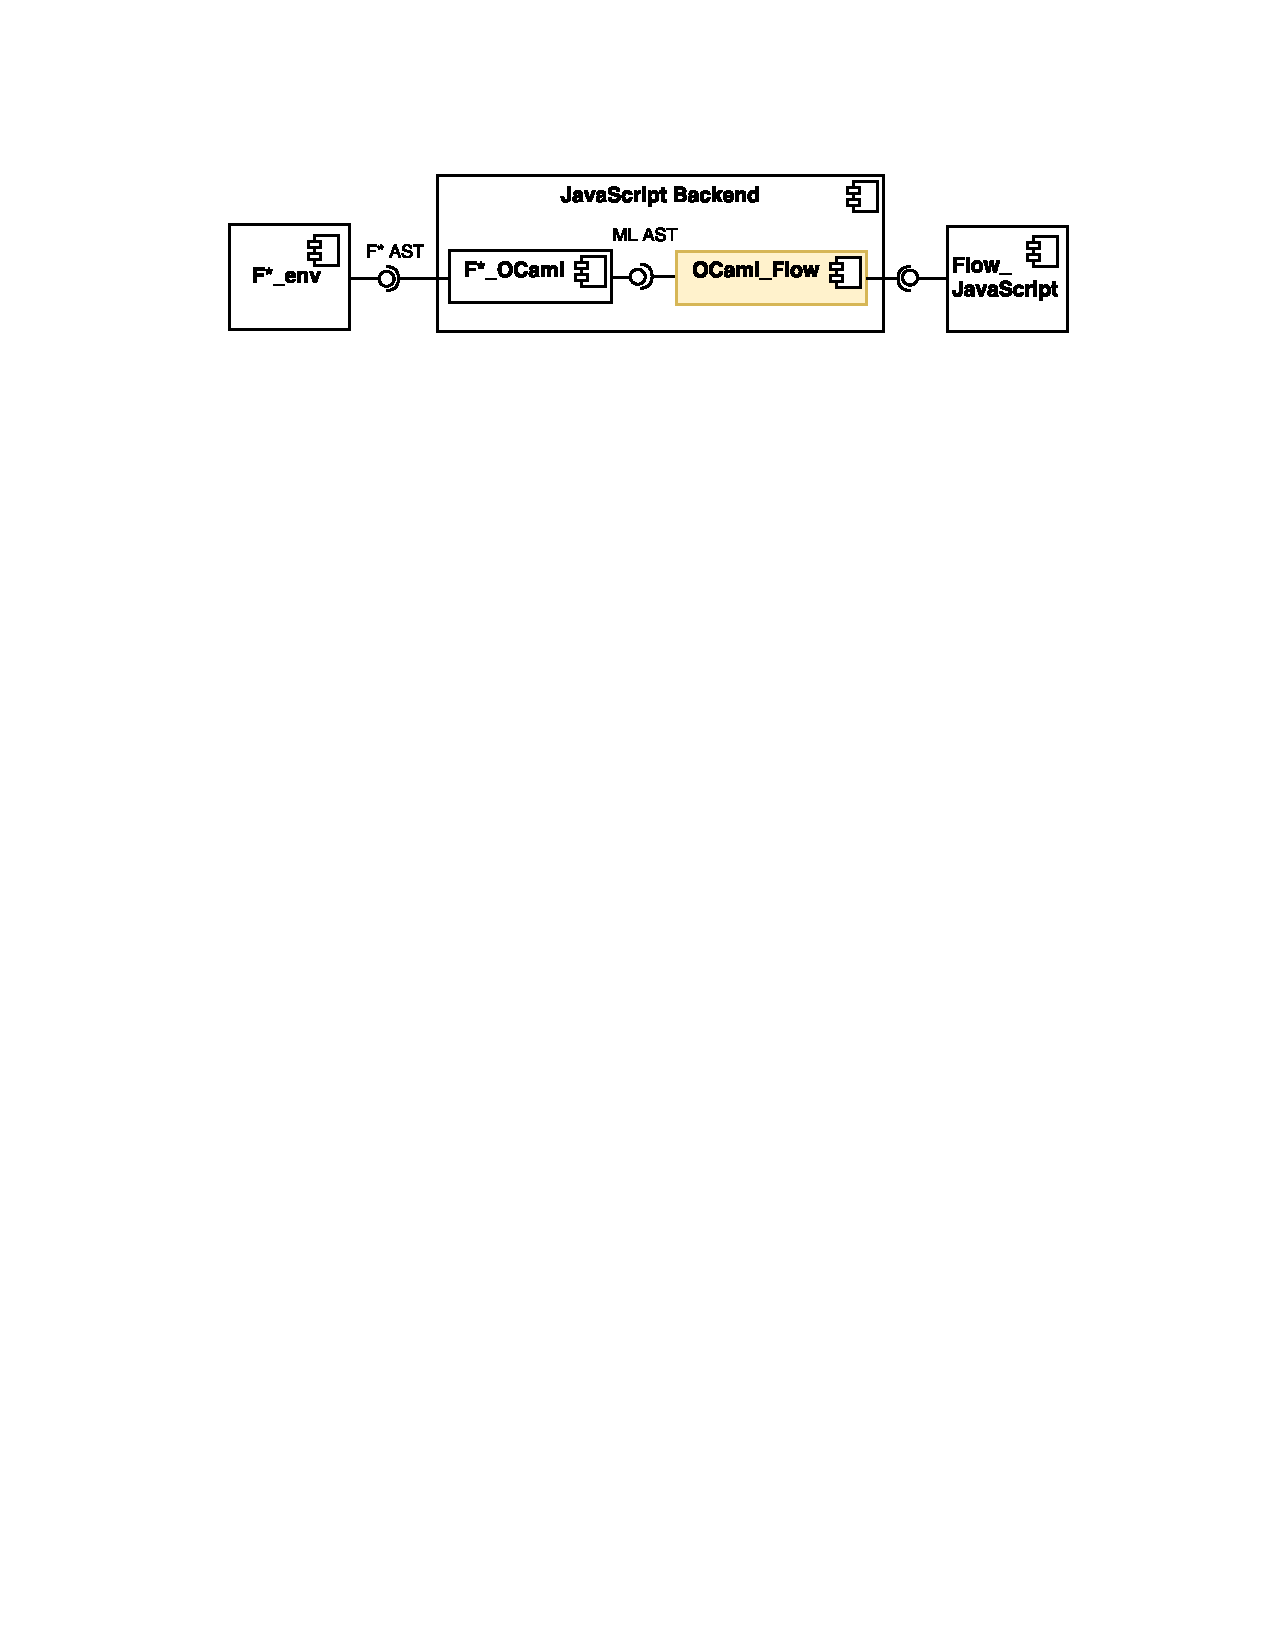
\includegraphics[width=0.8\textwidth]{DiagComp}
\caption{Диаграмма компонентов реализованного инструмента}
\label{fig:arch_js} 
\end{center}
\end{figure}

Ниже представлено описание каждого компонента.

Компонент \textit{F*\_env} отвечает за верификацию программы. Инструмент F* позволяет создавать программы и их верифицировать. Для того чтобы можно было их выполнять, необходим механизм извлечения верифицированного кода в программу на другом языке программирования. В проекте FStarLang такой механизм реализован для языка OCaml, схожий с~\cite{Letouzey2008}. Данный механизм удаляет зависимые и уточняющие типы, заменяя их стандартными типами целевого языка, ghost-вычисления и доказательства лемм, оставляя только их формулировки.

Компонент \textit{JavaScript Backend} состоит из двух компонентов: \textit{F*\_OCaml} и \textit{OCaml\_ \\Flow}. Компонент \textit{F*\_OCaml} отвечает за построение ML AST из F* AST, которое можно переиспользовать для создания новых бэкендов для инструмента F*. Ранее в проекте для старой версии инструмента использовался другой подход, а именно, трансляция языка F* в JavaScript напрямую~\cite{fully_abstract_js}. Компонент \textit{OCaml\_Flow} отвечает за трансляцию ML AST в Flow AST с сохранением аннотаций типов. Результатом работы компонента \textit{JavaScript Backend} является программа, которая может быть проверена инструментом Flow.

Компонент \textit{Flow\_JavaScript} необходим для получения JavaScript-приложения, которое может быть выполнено на программной платформе Node.js~\cite{node_js}. Данный компонент отвечает за удаление аннотаций типов и преобразование ES-стиля для работы с модулями в стиль CommandJS. Данное преобразование происходит с использованием соответствующих плагинов~\cite{flow_plugin} и~\cite{module_plugin}.

\subsection{Процесс построения JavaScript-приложения из F*-программы}

Пошаговый процесс получения JavaScript-приложения из F*-программы описан ниже (см. рис.~\ref{fig:modules}).

\begin{itemize}
\item \textbf{Шаг 0:} На вход подается F*-программа, которая может состоять из нескольких модулей. 
\item \textbf{Шаг 1:} Для каждого модуля программы происходит построение F* AST.
\item \textbf{Шаг 2:} Построение ML AST из F* AST путем удаления зависимых и уточняющих типов в F* AST, ghost-вычислений.
\item \textbf{Шаг 3:} Трансляция ML AST в Flow AST с сохранением аннотаций для типов.
\item \textbf{Шаг 4:} Получение программы, которая может быть проверена инструментом Flow. Количество модулей программы равняется количеству модулей исходной программы плюс количество модулей тех библиотек, чьи функции были использованы при создании программы. 
\item \textbf{Шаг 5:} Преобразование Flow-программы в JavaScript-программу (удаляется информация о типах, преобразование ES-стиль в CommandJS-стиль).
\end{itemize}

\begin{figure}[h!]
\begin{center}
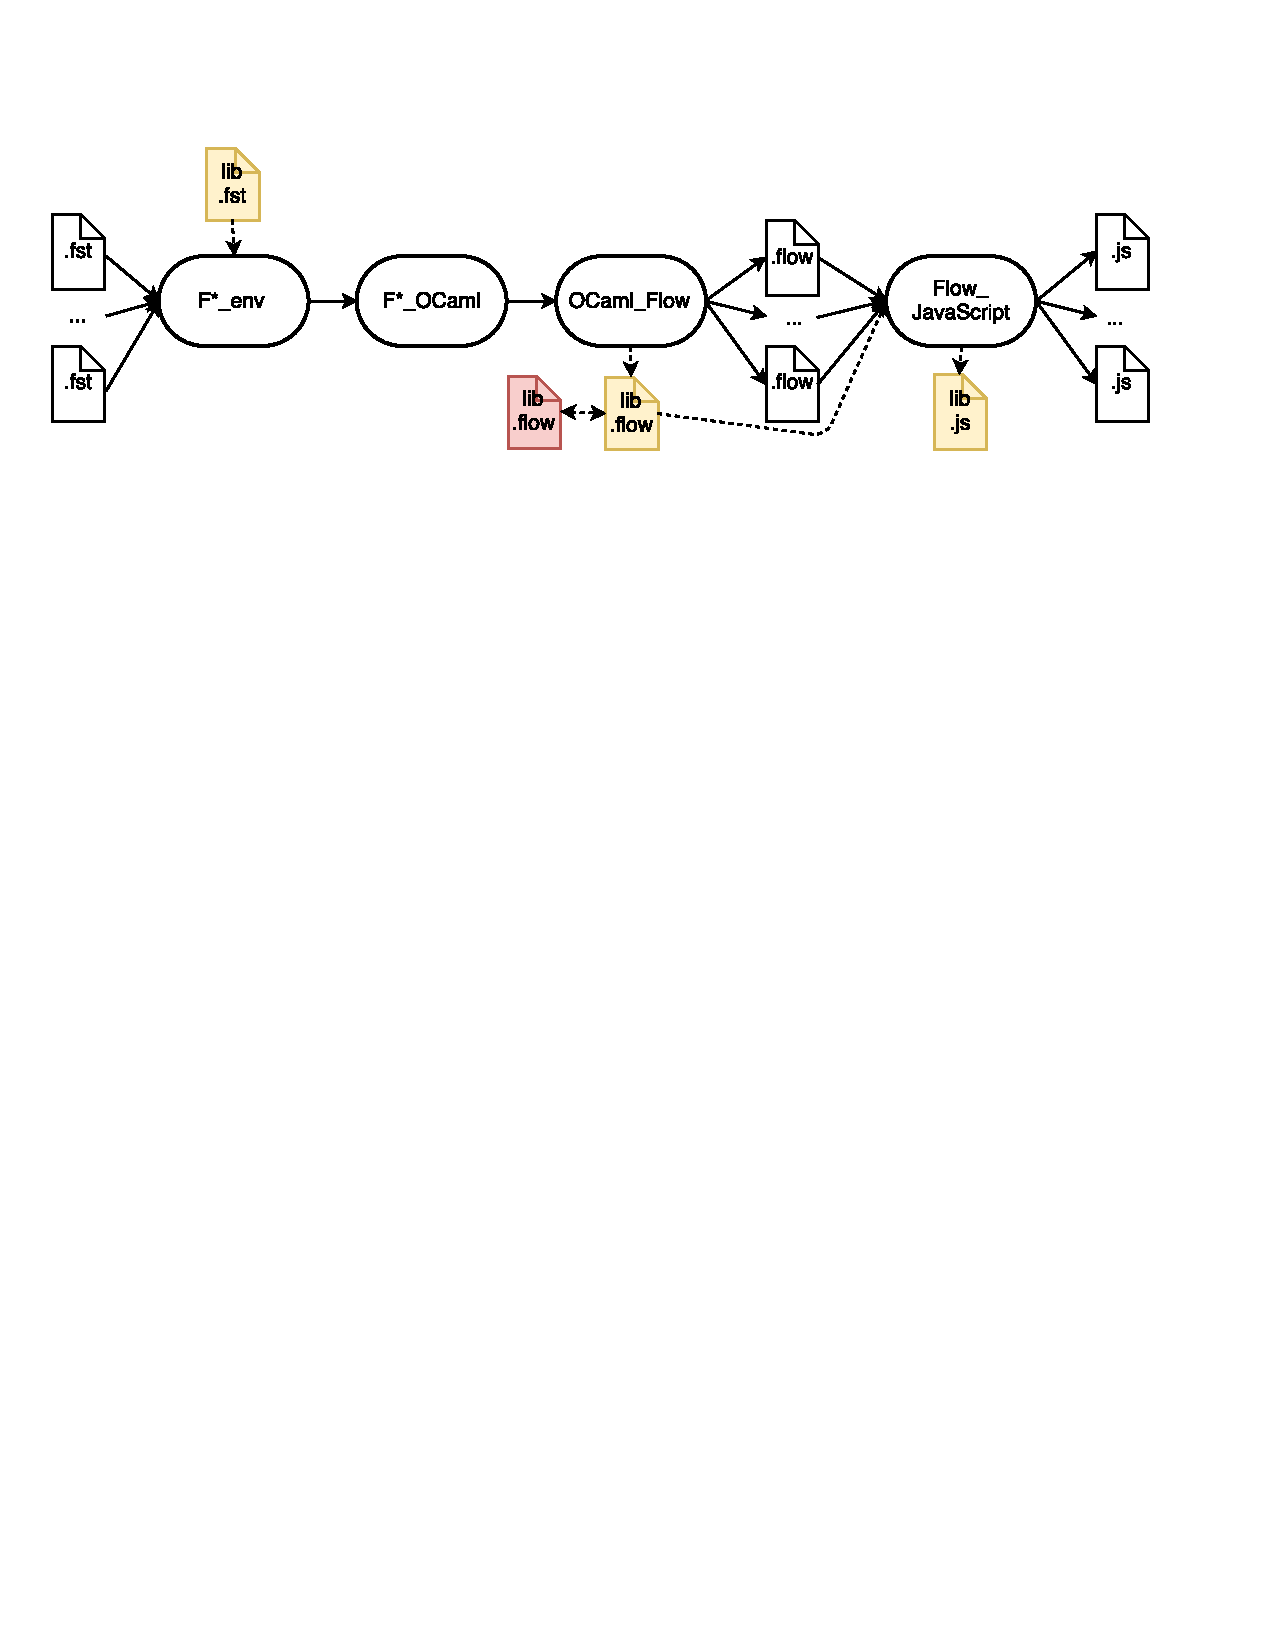
\includegraphics[width=\textwidth]{Workflow}
\caption{Процесс построения JavaScript-приложения из F*-программы}
\label{fig:modules} 
\end{center}
\end{figure}

\subsection{Работа с библиотечными функциями}

Программа чаще всего состоит из нескольких модулей и использует библиотечные функции. В F* такие библиотечные функции уже проверифицированы, что упрощает доказательства многих программ. По умолчанию при трансляции F*-программ происходит трансляция каждого модуля и модулей тех библиотек, которые были использованы при создании программы. Однако реализация таких библиотек не предназначена для быстрого выполнения программы, поэтому разработчик может заменить ее на более быструю, использовав функции целевого языка. Ответственность за такую замену полностью лежит на разработчике. Для того чтобы избежать большего количества ошибок, данную замену необходимо осуществлять так, чтобы была возможность проверить, используя инструмент Flow, согласованность написанной библиотеки с извлеченной из F* программой, например, с точки зрения системы типов целевого языка. На рис.~\ref{fig:modules} библиотека, которая была получена в результате трансляции соответствующих модулей F*-библиотек, отмечена желтым цветом (и соответствующие файлы имеют расширение .flow). Красным цветом отмечена библиотека, которая содержит в себе эффективную реализацию функций, использующую возможности целевого языка. 

\subsection{Взаимодействие с модулями}

Инструмент Flow поддерживает два стиля для работы с модулями, а именно, ES-стиль и CommandJS-стиль. В первом стиле используются конструкции  $export/import$, а во втором --- конструкции $require/exports$. При этом для типов осуществлена поддержка только ES-стиля, в то время как для переменных и функций поддержаны оба стиля ES и CommandJS. В данной работе для унификации трансляции использовался ES-стиль. Однако на данный момент он не поддерживается программной платформой Node.js~\cite{node_js}, поэтому для последнего преобразования необходим плагин, который ES-стиль заменяет на CommandJS-стиль.

\section{Экспериментальное исследование}

Экспериментальное исследование организовано в соответствии с методом Goal Question Metric~\cite{van2002goal}. Этот метод описывает модель эксперимента, которая имеет иерархическую структуру и состоит из трех уровней. На первом уровне необходимо определить \textit{цель} эксперимента, а также \textit{тестовые данные} (evaluation objects), на которых будут проводиться эксперименты. На втором уровне необходимо сформулировать \textit{вопросы}, которые помогут определить, достигнута ли поставленная цель или нет. На последнем уровне необходимо для каждого вопроса привести \textit{метрики}, помогающие ответить на поставленные вопросы. 

\textit{Целью} данного исследования является проверка эффективности реализованного инструмента для компиляции верифицированных F*-программ в робастные Веб-приложения. В качестве evaluation object использовался проект HACL*~\cite{hacl_star}. Для достижения поставленной цели были сформулированы следующие \textit{вопросы}.

\begin{itemize}
\item[] \textbf{Вопрос 1}. Каково качество кодогенератора в JavaScript?
\item[] \textbf{Вопрос 2}. Какова эффективность результатов трансляции из F* в JavaScript?
\item[] \textbf{Вопрос 3}. Какова готовность инструмента для использования в индустрии?
\end{itemize}

Для ответа на первый вопрос были сформулированы следующие \textit{метрики}.

\begin{itemize}
\item[] \textit{М1.1}. Количество верхнеуровневых функций в программе, которая получена в результате трансляции F*-программы в OCaml, и в программе, которая получена в результате трансляции F*-программы в JavaScript (Flow): F*\_OCaml и F*\_Flow.
\item[] \textit{М1.2}. Количество строк кода: F*\_OCaml и F*\_Flow.
\end{itemize}

Для ответа на второй вопрос использовалась следующая \textit{метрика}.

\begin{itemize}
\item[] \textit{М2.1}. Сравнение времени выполнения работы программ, одна из которых получена в результате трансляции F*-программы в JavaScript, а другая --- сразу создавалась на языке JavaScript: F*\_JavaScript и JavaScript.
\end{itemize}

Для ответа на последний вопрос были выбраны следующие \textit{метрики}.

\begin{itemize}
\item[] \textit{М3.1}. Количество библиотечных функций F*, которые необходимо реализовать на JavaScript для полноценной работы оттранслированной программы. 
\item[] \textit{М3.2}. Конструкции языка F*, которые не поддержаны.
\end{itemize}

Данная апробация проходила на машине со следующими характеристиками и окружением:

\begin{itemize}
\item OS: Windows 10 Pro x64;
\item Processor: Intel(R) Core(TM) i7-7500 CPU @ 2.70GHz;
\item RAM: 16 Gb;
\item OCaml 4.02.3, Cygwin\_x86\_64;
\item Node.js v7.2.1, Flow 0.38.0.
\end{itemize}

Для ответа на первый вопрос использовалась реализация алгоритма Chacha20~\cite{chacha} проекта HACL*. Для ее верификации использовалось около 37 библиотечных и вспомогательных модулей. Результаты измерений, сделанных согласно предложенным метрикам, приведены в таблице~\ref{tbl:metrics2}. 

\begin{center}  
\begin{tabular}{ | c | c | c | c | }
    \hline
      & F* & F*\_OCaml & F*\_Flow \\ \hline
    Кол-во верхнеуровневых функций & 32 & 32 & 32 \\ \hline
    Кол-во строк кода & 786 & 422 & 316 \\
    \hline
\end{tabular}
\captionsetup{type=table}
\captionof{table}{Результаты измерений, полученных по метрикам $M1.1$ и $M1.2$}
\label{tbl:metrics2} 
\end{center}

Программы F*\_OCaml и F*\_Flow  имеют меньшее количество строк кода, чем в исходной, потому что в ней использовалось около 9 лемм, которые при трансляции сохраняют только свою сигнатуру (см. листинги~\ref{lst:fact3} и~\ref{lst:fact4}). При этом имена переменных исходной программы сохраняются в оттранслированных программах.

Для ответа на второй вопрос использовалась реализация алгоритма СhaСha20. Первая программа была получена в результате применения разработанного в рамках данной работы инструмента для компиляции F*-программы в JavaScript, где исходная программа была взята из репозитория проекта HACL*. Описательные характеристики ее приведены в первом вопросе. Вторая программа была взята из репозитория~\cite{chachajs}, в которой 257 строк кода. График сравнения времени выполнения программ JavaScript и F*\_JavaScript приведен на рис.~\ref{fig:comparison}.

\begin{figure}[h!]
\begin{center}
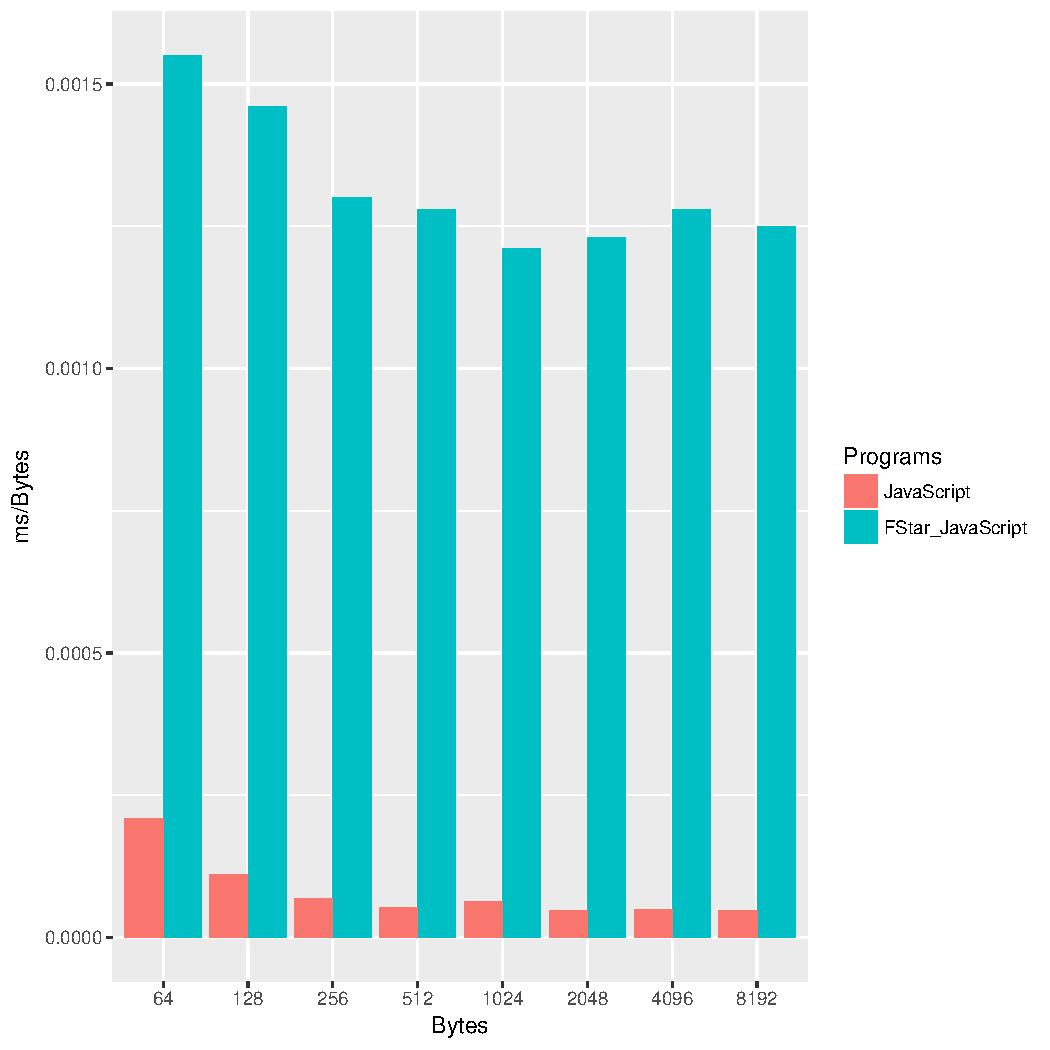
\includegraphics[width=.9\textwidth]{Comparison}
\caption{График сравнения времени выполнения программ JavaScript и F*\_JavaScript}
\label{fig:comparison} 
\end{center}
\end{figure}

Выполнялось измерение времени работы функции $encrypt$, результатом которой является зашифрованный текст, полученный по исходному тексту произвольной длины, 256-bit ключу, 96-bit случайному коду (nonce) и 32-bit счетчику. Сообщения были получены с использованием функции $crypto.randomBytes(len)$ из JavaScript-библиотеки $crypto$, где $len$ -- размер сообщения. Функция $encrypt$ запускалась 3000 раз на одних и тех данных, после чего бралось среднее время выполнения этой функции в миллисекундах. На графике представлены измерения для сообщений, которые имели размер, соответственно, 64 байт, 128 байт, 256 байт, 512 байт, 1 КБайт, 2 КБайт, 4 КБайт и 8 КБайт. Значения даны в миллисекундах на байт, то есть среднее время выполнения функции $encrypt$ было разделено на размер сообщения.

Данный график показывает, что время выполнения работы программы JavaScript превосходит время выполнения работы программы F*\_JavaScript. Данный факт объясняется тем, что в рамках данной работы выполнен только прототип инструмента, для которого в будущем будет проведен ряд оптимизаций. Например, замена оттранслированных функций на функции из целевого языка. С другой стороны, целью работы было создание безопасного и проверифицированного кода, что как известно, отражается на производительности программы. Одним из дальнейших направлений данной работы является реализация инструмента для компиляции F*-программы в JavaScript + WebAssembly~\cite{wasm}. Инструмент WebAssembly позволяет создавать быстрый и безопасный код, который можно использовать для совместной компиляции c JavaScript. При этом компиляция F*-кода в WebAssembly происходит с использованием KreMLin, который является промежуточным языком при трансляции подмножества языка F* в C. 

Точного ответа дать на последний вопрос нельзя, так как язык F* активно развивается и разрабатывается. На текущий момент реализована только та часть библиотечных функций на JavaScript, которая активно использовалась в проводимых экспериментах и без которой нельзя было бы получить готовое приложение. Так как при трансляции программы происходит трансляция модулей библиотек, чьи функции использовались при создании и верификации программы, то работоспособность оттранслированных функций в JavaScript зависела от того, какую реализацию для них предоставил механизм извлечения F*-программы в OCaml. Конструкции языка F*, которые не были поддержаны в данной работы: исключения (Exceptions) и автогенерация конструкторов. Их поддержка будет добавлена при необходимости. 


\section*{Заключение}
При выполнении данной работы были получены следующие результаты:
\begin{itemize}
\item сформулированы правила трансляции с языка F* на JavaScript, гарантирующие сохранение аннотаций типов;
\item выполнена реализация предложенного подхода на языке F*. Исходный код реализованного инструмента доступен по ссылке {\small \url{https://github.com/FStarLang/FStar/tree/polubelova_backends}}, автор принимал участие под учетной записью polubelova;
\item проведено экспериментальное исследование реализованного инструмента на примерах из криптографической библиотеки HACL*.
\end{itemize}

В дальнейшем планируется добавить возможность компиляции F*-программ в WebAssembly + JavaScript приложения и доказать корректность такой компиляции. Также планируется провести апробацию полученного инструмента на криптографической библиотеке HACL*, для которой нужно будет реализовать F*-библиотеки, используемые при верификации программ, на языке JavaScript.


\setmonofont[Mapping=tex-text]{CMU Typewriter Text}
\bibliographystyle{ugost2008ls}
\bibliography{diploma.bib}
%\nocite{*}
\end{document}